%% For double-blind review submission, w/o CCS and ACM Reference (max submission space)
\documentclass[acmsmall,review,anonymous]{acmart}\settopmatter{printfolios=true,printccs=false,printacmref=false}
%% For double-blind review submission, w/ CCS and ACM Reference
%\documentclass[acmsmall,review,anonymous]{acmart}\settopmatter{printfolios=true}
%% For single-blind review submission, w/o CCS and ACM Reference (max submission space)
%\documentclass[acmsmall,review]{acmart}\settopmatter{printfolios=true,printccs=false,printacmref=false}
%% For single-blind review submission, w/ CCS and ACM Reference
%\documentclass[acmsmall,review]{acmart}\settopmatter{printfolios=true}
%% For final camera-ready submission, w/ required CCS and ACM Reference
%\documentclass[acmsmall]{acmart}\settopmatter{}


%% Journal information
%% Supplied to authors by publisher for camera-ready submission;
%% use defaults for review submission.
% \acmJournal{PACMPL}
% \acmVolume{1}
% \acmNumber{CONF} % CONF = POPL or ICFP or OOPSLA
% \acmArticle{1}
% \acmYear{2018}
% \acmMonth{1}
% \acmDOI{} % \acmDOI{10.1145/nnnnnnn.nnnnnnn}
% \startPage{1}

%% Copyright information
%% Supplied to authors (based on authors' rights management selection;
%% see authors.acm.org) by publisher for camera-ready submission;
%% use 'none' for review submission.
\setcopyright{none}
%\setcopyright{acmcopyright}
%\setcopyright{acmlicensed}
%\setcopyright{rightsretained}
%\copyrightyear{2018}           %% If different from \acmYear

%% Bibliography style
\bibliographystyle{ACM-Reference-Format}
%% Citation style
%% Note: author/year citations are required for papers published as an
%% issue of PACMPL.
\citestyle{acmauthoryear}   %% For author/year citations


% %% Some recommended packages.
% \usepackage{booktabs}   %% For formal tables:
%                         %% http://ctan.org/pkg/booktabs
\usepackage{subcaption} %% For complex figures with subfigures/subcaptions
                        %% http://ctan.org/pkg/subcaption
\usepackage{wrapfig}

\usepackage{placeins}

\usepackage{todonotes}

\usepackage{ifthen}
\usepackage{pgf}
\usepackage{ulem}
\usepackage{tikz}
\usepackage{tikzpeople}
\usetikzlibrary{backgrounds}
\usetikzlibrary{fit}
\usetikzlibrary{calc}
\usetikzlibrary{positioning}
\usetikzlibrary{patterns}
\usetikzlibrary{decorations.pathreplacing}
\usetikzlibrary{arrows,shapes}
\usepackage{amssymb}

% Active adversary
\newcommand{\actadv}[4][]{
  \ifthenelse{\equal{#1}{}}{
    \draw[fill=white] #2 rectangle #3 node[pos=.5] {};
    \draw ($#2 + (2.25,1.5)$) node[devil,mirrored,minimum size=1cm] {};
    \draw[fill=white, fill opacity=0.5] #2 rectangle #3 node[pos=.5] {};
    \draw #2 rectangle #3 node[pos=.5,align=center] {\footnotesize #4};
  }{
    \onlyenv<#1>
    \draw[fill=white] #2 rectangle #3 node[pos=.5] {};
    \draw ($#2 + (3,1.5)$) node[devil,mirrored,minimum size=1cm] {};
    \draw[fill=white, fill opacity=0.5] #2 rectangle #3 node[pos=.5] {};
    \draw #2 rectangle #3 node[pos=.5] {\footnotesize #4};
    \endonlyenv
  }
}

% Inactive adversary
\newcommand{\inactadv}[4][]{
  \ifthenelse{\equal{#1}{}}{
    \draw[fill=white] #2 rectangle #3 node[pos=.5] {};
    \draw ($#2 + (2.25,1.5)$) node[devil,mirrored,minimum size=1cm] {};
    \draw[fill=white, fill opacity=0.4] #2 rectangle #3 node[pos=.5] {};
    \draw[fill=gray, fill opacity=0.5] #2 rectangle #3 node[pos=.5] {};
    \draw #2 rectangle #3 node[pos=.5] {\footnotesize #4};
  }{
    \onlyenv<#1>
    \draw[fill=white] #2 rectangle #3 node[pos=.5] {};
    \draw ($#2 + (3,1.5)$) node[devil,mirrored,minimum size=1cm] {};
    \draw[fill=white, fill opacity=0.4] #2 rectangle #3 node[pos=.5] {};
    \draw[fill=gray, fill opacity=0.5] #2 rectangle #3 node[pos=.5] {};
    \draw #2 rectangle #3 node[pos=.5] {\footnotesize #4};
    \endonlyenv
  }
}

% Active stack frame
\newcommand{\actsf}[4][]{
  \ifthenelse{\equal{#1}{}}{
    \draw[fill=white] #2 rectangle #3 node[pos=.5] {\footnotesize #4};
  }{
   \draw<#1>[fill=white] #2 rectangle #3 node[pos=.5] {#4};
 }
}

% Inactive stack frame
\newcommand{\inactsf}[4][]{
  \ifthenelse{\equal{#1}{}}{
    \draw[fill=white] #2 rectangle #3 node[pos=.5] {};
    \draw[fill=gray, fill opacity=0.5] #2 rectangle #3 node[pos=.5] {};
    \draw #2 rectangle #3 node[pos=.5] {\footnotesize #4};
  }{
    \draw<#1>[fill=white] #2 rectangle #3 node[pos=.5] {};
    \draw<#1>[fill=gray, fill opacity=0.5] #2 rectangle #3 node[pos=.5] {};
    \draw<#1> #2 rectangle #3 node[pos=.5] {\footnotesize #4};
  }
}

\newcommand{\capbrace}[3][sp1]{
  \draw [decorate,decoration={brace,amplitude=10pt,mirror,raise=4pt},yshift=0pt]
  #2 -- #3 node[draw=black] (#1) [black,midway,xshift=0.8cm] {};

}

\newcommand{\stdstackstart}{
  \scope
    \clip (-.1,-.1) rectangle (4.6,11.1);
    \fill[fill=white] (0,0) rectangle (4.5,11);
    \draw (0,0) -- (0,11);
    \draw (4.5,0) -- (4.5,11);
    \draw[fill=gray!50] (0,-.5) rectangle (4.5,2)
    node[pos=.5,color=black,align=center,yshift=0.1cm] {\footnotesize Higher
      stack\\\footnotesize frames...};
  \endscope
  % \draw[->] (-2,0) -- node[midway,sloped,above] {stack grows upward} (-2,15);
  \draw (-1.5,0) node {};
  \draw (-1.5,15) node {};
}


% stolen from https://tex.stackexchange.com/questions/14225/is-there-the-easiest-way-to-toggle-show-hide-navigational-grids-in-tikz/14230
\makeatletter
\newif\if@showgrid@grid
\newif\if@showgrid@left
\newif\if@showgrid@right
\newif\if@showgrid@below
\newif\if@showgrid@above
\tikzset{%
    every show grid/.style={},
    show grid/.style={execute at end picture={\@showgrid{grid=true,#1}}},%
    show grid/.default={true},
    show grid/.cd,
    labels/.style={font={\sffamily\small},help lines},
    xlabels/.style={},
    ylabels/.style={},
    keep bb/.code={\useasboundingbox (current bounding box.south west) rectangle (current bounding box.north west);},
    true/.style={left,below},
    false/.style={left=false,right=false,above=false,below=false,grid=false},
    none/.style={left=false,right=false,above=false,below=false},
    all/.style={left=true,right=true,above=true,below=true},
    grid/.is if=@showgrid@grid,
    left/.is if=@showgrid@left,
    right/.is if=@showgrid@right,
    below/.is if=@showgrid@below,
    above/.is if=@showgrid@above,
    false,
}

\def\@showgrid#1{%
    \begin{scope}[every show grid,show grid/.cd,#1]
    \if@showgrid@grid
    \begin{pgfonlayer}{background}
    \draw [help lines]
        (current bounding box.south west) grid
        (current bounding box.north east);
%
    \pgfpointxy{1}{1}%
    \edef\xs{\the\pgf@x}%
    \edef\ys{\the\pgf@y}%
    \pgfpointanchor{current bounding box}{south west}
    \edef\xa{\the\pgf@x}%
    \edef\ya{\the\pgf@y}%
    \pgfpointanchor{current bounding box}{north east}
    \edef\xb{\the\pgf@x}%
    \edef\yb{\the\pgf@y}%
    \pgfmathtruncatemacro\xbeg{ceil(\xa/\xs)}
    \pgfmathtruncatemacro\xend{floor(\xb/\xs)}
    \if@showgrid@below
    \foreach \X in {\xbeg,...,\xend} {
        \node [below,show grid/labels,show grid/xlabels] at (\X,\ya) {\X};
    }
    \fi
    \if@showgrid@above
    \foreach \X in {\xbeg,...,\xend} {
        \node [above,show grid/labels,show grid/xlabels] at (\X,\yb) {\X};
    }
    \fi
    \pgfmathtruncatemacro\ybeg{ceil(\ya/\ys)}
    \pgfmathtruncatemacro\yend{floor(\yb/\ys)}
    \if@showgrid@left
    \foreach \Y in {\ybeg,...,\yend} {
        \node [left,show grid/labels,show grid/ylabels] at (\xa,\Y) {\Y};
    }
    \fi
    \if@showgrid@right
    \foreach \Y in {\ybeg,...,\yend} {
        \node [right,show grid/labels,show grid/ylabels] at (\xb,\Y) {\Y};
    }
    \fi
    \end{pgfonlayer}
    \fi
    \end{scope}
}
\makeatother


 	
%%% Local Variables:
%%% TeX-master: "paper"
%%% End:

% Math packages
\usepackage{amsmath,amsfonts,amssymb,amsthm}
\usepackage{mathrsfs}
\usepackage{thmtools}
\usepackage{array}
\usepackage{cleveref}
\usepackage{stmaryrd}
\usepackage{mathpartir}


% Command control packages
\usepackage{ifthen}
\usepackage{ifpdf}

% Listings
\usepackage{listings}
\lstset{
  basicstyle=\ttfamily,
  columns=fullflexible,
  keepspaces=true,
  mathescape
}


% Tikz
\usepackage{tikz}

%%% Comments
% Comments
\newcommand\lau[1]{{\color{purple} \sf \footnotesize {LS: #1}}\\}
\newcommand\dominique[1]{{\color{purple} \sf \footnotesize {DD: #1}}\\}
\newcommand\lars[1]{{\color{purple} \sf \footnotesize {LB: #1}}\\}

%%% Math environments
\declaretheorem[numbered=yes,name=Lemma,qed=$\blacksquare$]{lemma}
\declaretheorem[numbered=yes,name=Theorem,qed=$\blacksquare$]{theorem}
\declaretheorem[numbered=yes,name=Definition,qed=$\blacksquare$]{definition}
\declaretheorem[numbered=yes,name=Specification,qed=$\blacksquare$]{specification}


%%% Math notation
\newcommand{\defeq}{\stackrel{\textit{\tiny{def}}}{=}}
\newcommand{\defbnf}{::=}
\newcommand{\sem}[1]{\left\llbracket #1 \right\rrbracket}
\newcommand{\ssem}[2][\Phi]{\sem{#2}_{\mathrm{src}}(#1)}
\newcommand{\tsem}[2][\Phi]{\sem{#2}_{\mathrm{trg}}(#1)}
\newcommand{\dom}{\mathrm{dom}}
\newcommand{\powerset}[1]{\mathcal{P}(#1)}

\newcommand{\npair}[2][n]{\left(#1,#2\right)}

\newcommand{\nsubeq}[1][n]{\overset{#1}{\subseteq}}
\newcommand{\nsupeq}[1][n]{\overset{#1}{\supseteq}}
\newcommand{\nequal}[1][n]{\overset{#1}{=}}

% Function arrows
\newcommand{\fun}{\rightarrow}
\newcommand{\parfun}{\rightharpoonup}
\newcommand{\monnefun}{\xrightarrow{\textit{\tiny{mon, ne}}}}



% Text
\newcommand{\tand}{\text{ and }}
\newcommand{\tor}{\text{ or }}
\newcommand{\totherwise}{\text{otherwise }}

% Equivalences
\newcommand{\sconeq}{\mathrel{\src{\approx_{\mathrm{ctx}}}}}
\newcommand{\tconeq}{\mathrel{\approx_{\mathrm{ctx}}}}

%%% Logical Relation notation
\newcommand{\typesetlr}[1]{\mathcal{#1}}
\newcommand{\lre}{\typesetlr{E}}
\newcommand{\lrexj}{\typesetlr{E}_{\var{xjmp}}}
\newcommand{\lrk}{\typesetlr{K}}
\newcommand{\lrr}{\typesetlr{R}}
\newcommand{\lro}{\typesetlr{O}}
\newcommand{\lrv}{\typesetlr{V}}
\newcommand{\lrp}{\typesetlr{P}}
\newcommand{\lrm}{\typesetlr{M}}

\newcommand{\stpair}[3][]{
\ifthenelse{\equal{#1}{}}
{\left(\src{#2_S},#3_T\right)}
{\left(\src{#2},#3\right)}}


\newcommand{\memSat}[3][n]{#2 :_{#1}#3}

\newcommand{\World}{\mathrm{World}}
\newcommand{\RegionName}{\mathrm{RegionName}}
\newcommand{\Region}{\mathrm{Region}}
\newcommand{\spatial}{\mathrm{spatial}}
\newcommand{\spatialo}{\mathrm{spatial\_owned}}
\newcommand{\pure}{\mathrm{pure}}
\newcommand{\revoked}{\mathrm{revoked}}
\newcommand{\State}{\mathrm{State}}
\newcommand{\Rels}{\mathrm{Rels}}
\newcommand{\UPred}[1]{\mathrm(#1)}

\newcommand{\future}{\sqsupseteq}
\newcommand{\pub}{\mathrm{pub}}
\newcommand{\privft}{\future^{\priv}}
\newcommand{\pubft}{\future^{\pub}}
\newcommand{\monprivnefun}{\xrightarrow[\text{\tiny{$\privft$}}]{\textit{\tiny{mon, ne}}}}
\newcommand{\monpubnefun}{\xrightarrow[\text{\tiny{$\pubft$}}]{\textit{\tiny{mon, ne}}}}

%%% Regions
\newcommand{\stdreg}[2]{\iota^{\mathrm{std},#2}_{#1}}
\newcommand{\stareg}[2][\stpair{\ms}{\ms}]{\iota^{\mathrm{sta},#2}_{#1}}
\newcommand{\spa}{\mathrm{s}}
\newcommand{\spao}{\mathrm{so}}
\newcommand{\pur}{\mathrm{p}}

%%% Instruction formatting
\newcommand{\sourcecolortext}{blue}
\newcommand{\sourcecolor}{\color{blue}}
\newcommand{\src}[1]{{\sourcecolor #1}}
\newcommand{\targetcolortext}{black}
\newcommand{\targetcolor}[1]{\color{black}}
\newcommand{\trg}[1]{{\targetcolor{} #1}}

\newcommand{\zinstr}[1]{\texttt{#1}}
\newcommand{\oneinstr}[2]{
  \ifthenelse{\equal{#2}{}}
  {\zinstr{#1}}
  {\zinstr{#1} \; #2}
}
\newcommand{\twoinstr}[3]{
  \ifthenelse{\equal{#2#3}{}}
  {\zinstr{#1}}
  {\zinstr{#1} \; #2 \; #3}
}
\newcommand{\threeinstr}[4]{
  \ifthenelse{\equal{#2#3#4}{}}
  {\zinstr{#1}}
  {\zinstr{#1} \; #2 \; #3 \; #4}
}

\newcommand{\fourinstr}[5]{
  \ifthenelse{\equal{#2#3#4#5}{}}
  {\zinstr{#1}}
  {\zinstr{#1} \; #2 \; #3 \; #4 \; #5}
}


%%% Source language
% No arguments
\newcommand{\sfail}{\zinstr{\src{fail}}}
\newcommand{\shalt}{\zinstr{\src{halt}}}
\newcommand{\sreturn}{\zinstr{\src{return}}}

% One argument
\newcommand{\sjmp}[1]{\oneinstr{\src{jmp}}{#1}}
\newcommand{\spush}[1]{\oneinstr{\src{push}}{#1}}
\newcommand{\spop}[1]{\oneinstr{\src{pop}}{#1}}

% Two arguments
\newcommand{\sjnz}[2]{\twoinstr{\src{jnz}}{#1}{#2}}
\newcommand{\sisptr}[2]{\twoinstr{\src{gettype}}{#1}{#2}}
\newcommand{\sgeta}[2]{\twoinstr{\src{geta}}{#1}{#2}}
\newcommand{\sgetb}[2]{\twoinstr{\src{getb}}{#1}{#2}}
\newcommand{\sgete}[2]{\twoinstr{\src{gete}}{#1}{#2}}
\newcommand{\sgetp}[2]{\twoinstr{\src{getp}}{#1}{#2}}
%\newcommand{\sgetloc}[2]{\twoinstr{\src{getloc}}{#1}{#2}}
\newcommand{\sgetlin}[2]{\twoinstr{\src{get}}{#1}{#2}}
\newcommand{\smove}[2]{\twoinstr{\src{move}}{#1}{#2}}
\newcommand{\sstore}[2]{\twoinstr{\src{store}}{#1}{#2}}
\newcommand{\sload}[2]{\twoinstr{\src{load}}{#1}{#2}}
\newcommand{\scca}[2]{\twoinstr{\src{cca}}{#1}{#2}}
\newcommand{\ssload}[2]{\twoinstr{\src{sload}}{#1}{#2}}
\newcommand{\sxjmp}[2]{\twoinstr{\src{xjmp}}{#1}{#2}}
\newcommand{\ssetatob}[2]{\twoinstr{\src{seta2b}}{#1}{#2}}
% scall - special two instruction
\newcommand{\scall}[4][]{  
\ifthenelse{\equal{#3#4}{}}
  {\ensuremath{\zinstr{\src{call}}_{#1}^{#2}}}
  {\ensuremath{\zinstr{\src{call}}_{#1}^{#2} \; #3 \; #4}}
}


% Three arguments
\newcommand{\srestrict}[3]{\threeinstr{\src{restrict}}{#1}{#2}{#3}}
\newcommand{\slt}[3]{\threeinstr{\src{lt}}{#1}{#2}{#3}}
\newcommand{\splus}[3]{\threeinstr{\src{plus}}{#1}{#2}{#3}}
\newcommand{\sminus}[3]{\threeinstr{\src{minus}}{#1}{#2}{#3}}
\newcommand{\scseal}[3]{\threeinstr{\src{cseal}}{#1}{#2}{#3}}
\newcommand{\ssplice}[3]{\threeinstr{\src{splice}}{#1}{#2}{#3}}


% Four arguments
%\newcommand{\ssubseg}[4]{\fourinstr{\src{subseg}}{#1}{#2}{#3}{#4}}
\newcommand{\ssplit}[4]{\fourinstr{\src{split}}{#1}{#2}{#3}{#4}}

%%% Target language
% No arguments
\newcommand{\tfail}{\zinstr{\trg{fail}}}
\newcommand{\thalt}{\zinstr{\trg{halt}}}

% One argument
\newcommand{\tjmp}[1]{\oneinstr{\trg{jmp}}{#1}}

% Two arguments
\newcommand{\tjnz}[2]{\twoinstr{\trg{jnz}}{#1}{#2}}
\newcommand{\tisptr}[2]{\twoinstr{\trg{gettype}}{#1}{#2}}
\newcommand{\tgeta}[2]{\twoinstr{\trg{geta}}{#1}{#2}}
\newcommand{\tgetb}[2]{\twoinstr{\trg{getb}}{#1}{#2}}
\newcommand{\tgete}[2]{\twoinstr{\trg{gete}}{#1}{#2}}
\newcommand{\tgetp}[2]{\twoinstr{\trg{getp}}{#1}{#2}}
%\newcommand{\tgetloc}[2]{\twoinstr{\trg{getloc}}{#1}{#2}}
\newcommand{\tgetlin}[2]{\twoinstr{\trg{getl}}{#1}{#2}}
\newcommand{\tmove}[2]{\twoinstr{\trg{move}}{#1}{#2}}
\newcommand{\tstore}[2]{\twoinstr{\trg{store}}{#1}{#2}}
\newcommand{\tload}[2]{\twoinstr{\trg{load}}{#1}{#2}}
\newcommand{\tcca}[2]{\twoinstr{\trg{cca}}{#1}{#2}}
\newcommand{\txjmp}[2]{\twoinstr{\trg{xjmp}}{#1}{#2}}
\newcommand{\tsetatob}[2]{\twoinstr{\trg{seta2b}}{#1}{#2}}

% Three arguments
\newcommand{\tsplice}[3]{\threeinstr{\trg{splice}}{#1}{#2}{#3}}
\newcommand{\trestrict}[3]{\threeinstr{\trg{restrict}}{#1}{#2}{#3}}
\newcommand{\tlt}[3]{\threeinstr{\trg{lt}}{#1}{#2}{#3}}
\newcommand{\tplus}[3]{\threeinstr{\trg{plus}}{#1}{#2}{#3}}
\newcommand{\tminus}[3]{\threeinstr{\trg{minus}}{#1}{#2}{#3}}
\newcommand{\tcseal}[3]{\threeinstr{\trg{cseal}}{#1}{#2}{#3}}

% Four arguments
%\newcommand{\tsubseg}[4]{\fourinstr{\trg{subseg}}{#1}{#2}{#3}{#4}}
\newcommand{\tsplit}[4]{\fourinstr{\trg{split}}{#1}{#2}{#3}{#4}}

%%% Domains
\newcommand{\plaindom}[1]{\mathrm{#1}}

\newcommand{\nats}{\mathbb{N}}
\newcommand{\ints}{\mathbb{Z}}

%%% Updates
\newcommand{\update}[2]{[#1 \mapsto #2]}
\newcommand{\updReg}[2]{\update{\reg.#1}{#2}}
\newcommand{\updPc}[1]{\Phi\updReg{\pcreg}{#1}}

%%% Source dom
\newcommand{\shareddom}[1]{\mathrm{#1}}
\newcommand{\RegName}{\shareddom{RegisterName}}
\newcommand{\Addr}{\shareddom{Addr}}
\newcommand{\Seal}{\shareddom{Seal}}
\newcommand{\Perm}{\shareddom{Perm}}
\newcommand{\Caps}{\shareddom{Cap}}
\newcommand{\SealableCaps}{\shareddom{SealableCap}}
\newcommand{\Word}{\shareddom{Word}}
\newcommand{\Instr}{\shareddom{Instr}}
\newcommand{\Mem}{\shareddom{Memory}}
\newcommand{\Reg}{\shareddom{RegisterFile}}
\newcommand{\Stk}{\shareddom{Stack}}
\newcommand{\Conf}{\shareddom{Conf}}
\newcommand{\ExecConf}{\shareddom{ExecConf}}
%\newcommand{\Global}{\shareddom{Global}}
\newcommand{\Linear}{\shareddom{Linear}}
\newcommand{\MemSeg}{\shareddom{MemorySegment}}
\newcommand{\StkFrame}{\shareddom{StackFrame}}
\newcommand{\Stack}{\shareddom{Stack}}

\newcommand{\scbnf}{\shareddom{sc}}
\newcommand{\cbnf}{\shareddom{c}}
\newcommand{\permbnf}{\shareddom{perm}}
\newcommand{\addrbnf}{\shareddom{a}}
\newcommand{\basebnf}{\shareddom{base}}
\newcommand{\aendbnf}{\shareddom{end}}
\newcommand{\rbnf}{\shareddom{r}}
%\newcommand{\glbnf}{\shareddom{gl}}
\newcommand{\linbnf}{\shareddom{l}}
\newcommand{\sealbasebnf}{\sigma_\shareddom{base}}
\newcommand{\sealendbnf}{\sigma_\shareddom{end}}

\newcommand{\sstk}{\shareddom{stk}}
\newcommand{\smsstk}{\shareddom{ms_{stk}}}
\newcommand{\sstkframe}{\shareddom{frame}}
\newcommand{\sopc}{\shareddom{opc}}
\newcommand{\sastk}{\shareddom{a_{stk}}}
\newcommand{\perm}{\var{perm}}
%\newcommand{\gl}{\var{g}}
\newcommand{\lin}{\var{l}}
\newcommand{\base}{\shareddom{base}}
\newcommand{\aend}{\shareddom{end}}
\newcommand{\addr}{\shareddom{a}}
\newcommand{\scap}{\shareddom{c}}
\newcommand{\sms}{\shareddom{ms}}

\newcommand{\stkptr}[1]{\mathrm{stack\text{-}ptr}(#1)}
\newcommand{\retptr}{\mathrm{ret\text{-}ptr}}
\newcommand{\retptrd}{\mathrm{ret\text{-}ptr\text{-}data}}
\newcommand{\retptrc}{\mathrm{ret\text{-}ptr\text{-}code}}

\newcommand{\seal}[1]{\shareddom{seal}(#1)}
\newcommand{\sealed}[1]{\shareddom{sealed}(#1)}

\newcommand{\failed}{\mathrm{failed}}
% DOMI: defining a macro named ``undefined'' breaks many latex packages.
%       (this is just another way that LaTeX is broken as a programming language)
% \newcommand{\undefined}{\mathrm{undefined}}
\newcommand{\tundefined}{\mathrm{undefined}}
\newcommand{\halted}{\mathrm{halted}}

%%% Target domain
\newcommand{\targetdom}[1]{\mathrm{#1}}
\newcommand{\tRegName}{\targetdom{RegisterName}}

%%% Programs and contexts
\newcommand{\program}{\mathscr{P}}
\newcommand{\context}{\mathscr{C}}

\newcommand{\plug}[2]{#1[#2]}

%%% Operational semantics
\newcommand{\step}{\rightarrow}
\newcommand{\nstep}[1][n]{\step_{#1}}
\newcommand{\steps}{\step^*}
\newcommand{\diverge}{{\Uparrow}}
\newcommand{\term}[1][-]{{\Downarrow_{#1}}}

%%% Variables
\newcommand{\var}[1]{\mathit{#1}}
\newcommand{\rn}{\var{rn}}
\newcommand{\reg}{\var{reg}}
\newcommand{\mem}{\var{mem}}
\newcommand{\ms}{\var{ms}}
\newcommand{\pc}{\var{pc}}
\newcommand{\stk}{\var{stk}}
\newcommand{\link}{\var{link}}
\newcommand{\stkf}{\stk_{\var{frame}}}
\newcommand{\ret}{\var{ret}}
\newcommand{\data}{\var{data}}
\newcommand{\code}{\var{code}}
\newcommand{\priv}{\var{priv}}
\newcommand{\opc}{\var{opc}}
\newcommand{\odata}{\var{odata}}
\newcommand{\vsc}{\var{sc}}
\newcommand{\cb}{\vsc}
\newcommand{\baddr}{\var{b}}
\newcommand{\eaddr}{\var{e}}
\newcommand{\aaddr}{\var{a}}
\newcommand{\stdrng}{[\baddr,\eaddr]}

%%% Constants
\newcommand{\constant}[1]{\mathrm{#1}}
\newcommand{\calllen}{\constant{call\_len}}
\newcommand{\stkb}{\constant{stk\_base}}

%%% Named registers
\newcommand{\pcreg}{\mathrm{pc}}
\newcommand{\rstk}{\mathrm{r}_\mathrm{stk}}
\newcommand{\rO}{\mathrm{r}_\mathrm{ret}}
\newcommand{\rret}{\rO}
\newcommand{\rretc}{\mathrm{r}_\mathrm{ret code}}
\newcommand{\rretd}{\mathrm{r}_\mathrm{ret data}}
\newcommand{\rdata}{\mathrm{r}_\mathrm{data}}
\newcommand{\rtmp}[1]{\mathrm{r}_\mathrm{t#1}}



%%% locality
%\newcommand{\plainlocality}[1]{\mathrm{#1}}
%\newcommand{\glob}{\plainlocality{global}}
%\newcommand{\local}{\plainlocality{local}}

%%% linearity
\newcommand{\plainlinearity}[1]{\mathrm{#1}}
\newcommand{\linear}{\plainlinearity{linear}}
\newcommand{\normal}{\plainlinearity{normal}}


%%% Permissions
\newcommand{\plainperm}[1]{\textsc{#1}}
%\newcommand{\rwlx}{\plainperm{rwlx}}
\newcommand{\rwx}{\plainperm{rwx}}
\newcommand{\rx}{\plainperm{rx}}
%\newcommand{\rwlxo}{\plainperm{rwlxo}}
%\newcommand{\rwlo}{\plainperm{rwlo}}
%\newcommand{\rwl}{\plainperm{rwl}}
%\newcommand{\rwxo}{\plainperm{rwxo}}
%\newcommand{\rwo}{\plainperm{rwo}}
\newcommand{\rw}{\plainperm{rw}}
%\newcommand{\rxo}{\plainperm{rxo}}
\newcommand{\readonly}{\plainperm{r}}
\newcommand{\ro}{\readonly}
\newcommand{\noperm}{\plainperm{0}}
%\newcommand{\nopermo}{\plainperm{0o}}
%\newcommand{\enter}{\plainperm{e}}
%\newcommand{\entero}{\plainperm{eo}}

%%% Braces
\newcommand{\comp}[1]{[#1]}

%%% Functions
\newcommand{\plainfun}[2]{
  \ifthenelse{\equal{#2}{}}
  {\mathit{#1}}
  {\mathit{#1}(#2)}
}

%\newcommand{\isLoc}[1]{\plainfun{isLocal}{#1}}
%\newcommand{\nonLoc}[1]{\plainfun{nonLocal}{#1}}
%\newcommand{\opaquePerm}[1]{\plainfun{opaquePerm}{#1}}
%\newcommand{\updPcPerm}[1]{\plainfun{updatePcPerm}{#1}}
%\newcommand{\writeLocalAllowed}[1]{\plainfun{writeLocalAllowed}{#1}}
\newcommand{\addressable}[1]{\plainfun{addressable}{#1}}
\newcommand{\callCond}[1]{\plainfun{callCondition}{#1}}
\newcommand{\decInstr}[1]{\plainfun{decodeInstruction}{#1}}
\newcommand{\decPerm}[1]{\plainfun{decodePerm}{#1}}
\newcommand{\encInstr}[1]{\plainfun{encodeInstruction}{#1}}
\newcommand{\encPerm}[1]{\plainfun{encocePerm}{#1}}
\newcommand{\encLin}[1]{\plainfun{encoceLin}{#1}}
\newcommand{\encType}[1]{\plainfun{encodeType}{#1}}
\newcommand{\exec}[1]{\plainfun{executable}{#1}}
\newcommand{\execCond}[1]{\plainfun{executeCondition}{#1}}
\newcommand{\isLinear}[1]{\plainfun{isLinear}{#1}}
\newcommand{\linCons}[1]{\plainfun{linearityConstraint}{#1}}
\newcommand{\noRetStkMs}[1]{\plainfun{noRetStk_{ms}}{#1}}
\newcommand{\noRetStkReg}[1]{\plainfun{noRetStk_{reg}}{#1}}
\newcommand{\nonExec}[1]{\plainfun{nonExecutable}{#1}}
\newcommand{\nonLinear}[1]{\plainfun{nonLinear}{#1}}
\newcommand{\nonZero}[1]{\plainfun{nonZero}{#1}}
\newcommand{\range}[1]{\plainfun{range}{#1}}
\newcommand{\readAllowed}[1]{\plainfun{readAllowed}{#1}}
\newcommand{\readCond}[1]{\plainfun{readCondition}{#1}}
\newcommand{\writeCond}[1]{\plainfun{writeCondition}{#1}}
\newcommand{\sealAss}[1]{\plainfun{sealAssignment}{#1}}
\newcommand{\updPcAddr}[1]{\plainfun{updatePc}{#1}}
\newcommand{\withinBounds}[1]{\plainfun{withinBounds}{#1}}
\newcommand{\writeAllowed}[1]{\plainfun{writeAllowed}{#1}}
\newcommand{\xjumpResult}[3]{\plainfun{xjumpResult}{#1,#2,#3}}

% Paper specific redefinitions of commands
\renewcommand{\MemSeg}{\shareddom{MemSeg}}
\renewcommand{\Reg}{\shareddom{RegFile}}
\renewcommand{\RegName}{\shareddom{RegName}}
\renewcommand{\decInstr}[1]{\plainfun{decode}{#1}}
\renewcommand{\updPcAddr}[1]{\plainfun{updPc}{#1}}
\renewcommand{\linCons}[1]{\plainfun{linClear}{#1}}
\renewcommand{\nonExec}[1]{\plainfun{nonExec}{#1}}
\newcommand{\xjmpres}[1]{\plainfun{xjmpRes}{#1}}

\begin{document}

%% Title information
\title{StackTokens: Enforcing Well-bracketed Control Flow and Stack Encapsulation using Linear Capabilities}
% \titlenote{with title note}
% \subtitle{Fully abstract overlay semantics}
% \subtitlenote{with subtitle note}

%% Author information
%% Contents and number of authors suppressed with 'anonymous'.
%% Each author should be introduced by \author, followed by
%% \authornote (optional), \orcid (optional), \affiliation, and
%% \email.
%% An author may have multiple affiliations and/or emails; repeat the
%% appropriate command.
%% Many elements are not rendered, but should be provided for metadata
%% extraction tools.

\author{Lau Skorstengaard}
% \orcid{nnnn-nnnn-nnnn-nnnn}             %% \orcid is optional
\affiliation{
  \institution{Aarhus~University}
  \country{Denmark}                    %% \country is recommended
}
\email{lask@cs.au.dk}

%% Author with two affiliations and emails.
\author{Dominique Devriese}
\orcid{0000-0002-3862-6856}             %% \orcid is optional
\affiliation{
  \institution{KU~Leuven}           %% \institution is required
  \country{Belgium}                   %% \country is recommended
}
\email{dominique.devriese@cs.kuleuven.be}         %% \email is recommended

\author{Lars Birkedal}
% \orcid{nnnn-nnnn-nnnn-nnnn}             %% \orcid is optional
\affiliation{
  \institution{Aarhus~University}
  \country{Denmark}                    %% \country is recommended
}
\email{birkedal@cs.au.dk}

\begin{abstract}
  We propose and study StackTokens: a new calling convention that provably enforces well-bracketed control flow and local state encapsulation on a capability machine.
  The calling convention is based on linear capabilities, a type of capabilities that are prevented from being duplicated by the hardware.
  In addition to designing and formalising this new calling convention, we also contribute a new way to formalise and prove that it effectively enforces well-bracketed control flow and local state encapsulation, using what we call a fully abstract overlay semantics.
\end{abstract}


% %% 2012 ACM Computing Classification System (CSS) concepts
% %% Generate at 'http://dl.acm.org/ccs/ccs.cfm'.
% \begin{CCSXML}
% <ccs2012>
% <concept>
% <concept_id>10011007.10011006.10011008</concept_id>
% <concept_desc>Software and its engineering~General programming languages</concept_desc>
% <concept_significance>500</concept_significance>
% </concept>
% <concept>
% <concept_id>10003456.10003457.10003521.10003525</concept_id>
% <concept_desc>Social and professional topics~History of programming languages</concept_desc>
% <concept_significance>300</concept_significance>
% </concept>
% </ccs2012>
% \end{CCSXML}

% \ccsdesc[500]{Software and its engineering~General programming languages}
% \ccsdesc[300]{Social and professional topics~History of programming languages}
%% End of generated code


\keywords{fully abstract compilation, secure compilation, capability machines, linear capabilities, well-bracketed control flow, stack frame encapsulation, overlay semantics}


\maketitle


\section{Introduction}
\label{sec:introduction}
Secure compilers preserve source-language (security-relevant) properties even when the compiled code interacts with arbitrary target-language components.
Generally, properties that hold in the source language but not in the target language need to be somehow enforced by the compiler.
Two properties that hold in many high-level source languages, but not in the assembly languages they are compiled to, are well-bracketed control flow and encapsulation of local state.

Well-bracketed control flow (WBCF) expresses that invoked functions must either return to their callers, invoke other functions themselves or diverge, and generally holds in programming languages that do not offer a primitive form of continuations. 
At the assembly level, this property does not hold immediately. 
Invoked functions get direct access to return pointers that they are supposed to jump to a single time at the end of their execution.
There is, however, no guarantee that untrusted assembly code respects this intended usage.
Particularly, a function may invoke return pointers from other stack frames than its own: either frames higher in the call stack or ones that no longer exist as they have already returned. 

Local state encapsulation (LSE) is the guarantee that when a function invokes another function, its local variables (saved on its stack frame) will not have been read or modified when the invoked function returns.
At the assembly level, this property also does not hold immediately.
The calling function's local variables are stored on the stack during the invocation, and functions are not supposed to touch stack frames other than their own.
However, untrusted assembly code is free to ignore this requirement and read or overwrite the local state of other stack frames.
To enforce these properties, target language security primitives are needed that can be used to prevent untrusted code from misbehaving, without imposing too much overhead on well-behaved code.
The virtual-memory based security primitives on commodity processors do not seem sufficiently fine-grained to efficiently support this.
More suitable security primitives are offered by a type of CPUs known as capability machines \citep{levy_capability-based_1984,watson_cheri:_2015}.
These processors use tagged memory to enforce a strict separation between integers and {\itshape capabilities}: pointers that carry authority.
Capabilities come in different flavours.
Memory capabilities allow reading from and writing to a block of memory.
Additionally, capability machines offer some form of {\itshape object capabilities} that represent low-level encapsulated closures, i.e. a piece of code coupled with private state that it gains access to upon invocation.
The concrete mechanics of object capabilities varies between different capability machines.
% KJAA: This 'sealed' and 'common seal' business is unclear to me.
On a recent capability machine called CHERI, for example, they take the form of pairs of capabilities that represent the code and data parts of the closure.
Each of the two capabilities are sealed with a common seal which make them opaque.
The hardware transparently unseals the pair upon invocation~\citep{watson_capability_2015}.

To enforce WBCF and LSE on a capability machine, there are essentially two approaches.
A first approach uses separate stacks for distrusting components, and a central, trusted stack manager component that mediates cross-component invocations.
This idea has been applied in CheriBSD (an operating system built on CHERI)~\citep{watson_capability_2015}, but it is not without downsides.
First, it scales poorly to large amounts of distrusting components, because of the need to reserve separate stack space for all components.
Also, in the presence of higher-order values (e.g. function pointers, objects etc.), the stack manager needs to be able to decide which component a higher-order value belongs to in order to provide it the right stack pointer upon invocation.
It is not clear how this can be done efficiently in the presence of large amounts of components.
Finally, this approach does not allow passing stack references between components.

A more scalable approach retains a single stack that is shared between components.
Enforcing WBCF and LSE in this approach requires a way to temporarily provide stack and return capabilities to an untrusted component, and to revoke them after it returns.
While capability revocation is expensive in general, some capability machines offer restricted forms of revocation that can be implemented efficiently.
For example, CHERI offers a form of {\itshape local} capabilities that, briefly, can only be stored in registers or on the stack, but not in other parts of memory.
\citet{skorstengaard_reasoning_2017} has demonstrated that by making the stack and return pointer local, and by introducing a number of security checks and measures, the two properties can be guaranteed.
% KJAA: 'Boundary crossing' is new here.
However, a problem with this approach is that revoking the local stack and return capabilities on every boundary crossing requires clearing the entire unused part of the stack, a potentially expensive operation.

In this work, we propose and study StackTokens: an alternative calling convention that enforces WBCF and LSE with a single shared stack.
Instead of CHERI's local capabilities, it builds on {\itshape linear} capabilities; a new form of capabilities that has not been previously described in the published literature.\footnote{Although they are mentioned here and there by different people.}
% KJAA: Perhaps make it clear by who and when/where?
These capabilities are non-duplicable, enforced by the hardware.
We propose to make stack and return pointers linear and require components to hand them out in cross-component invocations and to return them in returns.
The non-duplicability of linear capabilities together with some security checks allow us to guarantee WBCF and LSE without large overhead on boundary crossings, particularly without the need for clearing large blocks of memory.

A second contribution of this work is the way in which we formulate these two properties, using a technique we call {\itshape fully abstract overlay semantics}.
Formulations in previous work are either partial and not suitable for reasoning~\cite{abadi_control-flow_2005} or lacked evidence of generality~\cite{skorstengaard_reasoning_2017}.
Our new formulation starts from the premise that security results for a calling convention should be reusable as part of a larger proof of a secure compiler.
To accomodate this, we define a second operational semantics for our target language, with a native well-bracketed stack and primitive ways to do calls and returns.
This well-behaved semantics guarantees WBCF and LSE natively for components using our calling convention.
As such, these components can be sure that they will only ever interact with other well-behaved components that respect our desired properties.
To express security of our calling convention, we then show that considering the same components in the original semantics does not give adversaries additional ways to interact with them. 
More formally, we show that mapping a component in the well-behaved semantics to the same component in the original semantics is fully abstract~\cite{abadi_protection_1999}, i.e. that components are indistinguishable to arbitrary adversaries in the well-behaved language iff they are indistinguishable to arbitrary adversaries in the original language.

This approach expresses what it means to enforce our desirable properties in a general way, and makes it clear that we can support a very general class of programs.
Additionally, formulating security of a calling convention in this way makes it potentially reusable in a larger security proof of a full compiler.
The idea is that security of such a compiler could be verified by proving fully abstract compilation with respect to the well-behaved semantics of the target language, so that the proof can rely on native well-bracketedness and local stack frame encapsulation.
This independent result could then be composed with our result to obtain security of the compiler targeting the real target language, by transitivity of full abstraction.

\todo[inline]{Add itemized contributions}

\paragraph{Outline} Blabla

% \begin{acks}                            %% acks environment is optional
%                                         %% contents suppressed with 'anonymous'
%   %% Commands \grantsponsor{<sponsorID>}{<name>}{<url>} and
%   %% \grantnum[<url>]{<sponsorID>}{<number>} should be used to
%   %% acknowledge financial support and will be used by metadata
%   %% extraction tools.
%   This material is based upon work supported by the
%   \grantsponsor{GS100000001}{National Science
%     Foundation}{http://dx.doi.org/10.13039/100000001} under Grant
%   No.~\grantnum{GS100000001}{nnnnnnn} and Grant
%   No.~\grantnum{GS100000001}{mmmmmmm}.  Any opinions, findings, and
%   conclusions or recommendations expressed in this material are those
%   of the author and do not necessarily reflect the views of the
%   National Science Foundation.
% \end{acks}

\section{A Capability Machine with Sealing and Linear Capabilities}
\label{sec:cap-mach-w-seal-and-lin}
\begin{itemize}
\item present our \emph{target language} and its operational semantics (excerpts)
\item mention roughly what components look like
\end{itemize}
\begin{figure}[htb]
  \centering
  \[
  \arraycolsep=1.4pt
  \begin{array}{rrcl l rrcl}
   \addrbnf,\basebnf \in & \Addr & \defeq & \nats & \phantom{mak} & \sealbasebnf, \sigma \in & \Seal & \defeq & \nats\\
    \permbnf \in& \Perm & \defbnf & \rwx \mid \rx \mid \rw \mid \ro \mid \noperm & & &\linbnf & \defbnf & \linear \mid \normal\\
    &\aendbnf & \in & \Addr \cup \{\infty \} & & &\sealendbnf & \in & \Seal \cup \{\infty \}\\
    \scbnf \in &\SealableCaps&\defbnf & \multicolumn{6}{l}{((\permbnf,\linbnf),\basebnf,\aendbnf,\addrbnf) \mid \seal{\sealbasebnf,\sealendbnf,\sigma}}\\
    \cbnf \in&\Caps& \defbnf &  \SealableCaps \mid \sealed{\sigma,\scbnf} & & w \in &\Word & \defeq & \ints \uplus \Caps\\ 
    \rbnf \in& \RegName & \defbnf & \multicolumn{6}{l}{\pcreg \mid \rretd \mid \rretc \mid \rstk \mid \rdata \mid \rtmp{1} \mid \rtmp{2} \mid \dots} \\
    &\Reg & \defeq & \RegName \fun \Word & & &\Mem & \defeq & \Addr \fun \Word\\
    &\MemSeg & \defeq & \Addr \parfun \Word & & \Phi \in & \ExecConf & \defeq & \Mem \times \Reg\\
    &\Conf & \defeq & \multicolumn{6}{l}{\ExecConf \cup \{\failed\} \cup \{\halted\} }
  \end{array}
\]
\[
  \arraycolsep=1.4pt
\begin{array}{rcl}
\multicolumn{3}{l}{    \arraycolsep=0pt
      \com{r} \in  \tRegName \hspace{2.5cm}   \com{\rn} \defbnf \com{r} \mid \nats
}\\
\Instr &\defbnf & \tfail \mid \thalt \mid \tjmp{\com{r}} \mid \tjnz{\com{r}}{\com{\rn}} \mid \tisptr{\com{r}}{\com{r}} \mid \tgeta{\com{r}}{\com{r}} \mid \tgetb{\com{r}}{\com{r}} \mid \tgete{\com{r}}{\com{r}}\mid\tgetp{\com{r}}{\com{r}} \mid\\
      & &    \tgetlin{\com{r}}{\com{r}} \mid \tmove{\com{r}}{\com{\rn}} \mid \tstore{\com{r}}{\com{r}} \mid \tload{\com{r}}{\com{r}} \mid \tcca{\com{r}}{\com{\rn}} \mid \trestrict{\com{r}}{\com{\rn}} \mid \tlt{\com{r}}{\com{\rn}}{\com{\rn}} \mid \\
  & & \tplus{\com{r}}{\com{\rn}}{\com{\rn}} \mid \tminus{\com{r}}{\com{\rn}}{\com{\rn}} \mid \tsetatob{\com{r}} \mid \txjmp{\com{r}}{\com{r}} \mid \tcseal{\com{r}}{\com{r}} \mid \tsplit{\com{r}}{\com{r}}{\com{r}}{\com{\rn}} \mid\\ 
      & & \tsplice{\com{r}}{\com{r}}{\com{r}} 
\end{array}
\]
  \caption{The syntax of our capbility machine with seals and linera capbilities.}
  \label{fig:target-syntax}
\end{figure}

\begin{figure}[h]
  \centering
  \[
    \Phi \step
  \begin{cases}
    \sem{\decInstr{\Phi.\mem(\aaddr)}}(\Phi) &
    \arraycolsep=0pt
      \begin{array}[t]{l}
        \text{if }\Phi(\pcreg) = ((\perm,\_),\baddr,\eaddr,\aaddr) \wedge
        \baddr \le \aaddr \le \eaddr \wedge \perm \in \{\rwx,\rx\}
      \end{array} \\
      \failed & \totherwise
  \end{cases}
\]
\[
  \updPcAddr{\Phi} =
  \begin{cases}
    \Phi\updReg{\pcreg}{w} & \Phi(\pcreg) = ((\perm,\lin),\baddr,\eaddr,\aaddr) \wedge w = ((\perm,\lin),\baddr,\eaddr,\aaddr+1)\\
    \Phi  & \totherwise
  \end{cases}
\]
\[
  \linCons{w} =
  \begin{cases}
    0 & \isLinear{w} \\
    w & \totherwise
  \end{cases}
\] 
\[
  \xjmpres{c_1,c_2,\Phi} =
  \begin{cases}
    \Phi\updReg{\pcreg}{c_1}\updReg{\rdata}{c_2} & \nonExec{c_2} \\
    \failed & \totherwise
  \end{cases}
\]
  \begin{tabular}{|>{$}c<{$}|>{$}p{3.4cm}<{$}|>{\raggedright\arraybackslash}p{7cm}|}
    \hline
    i \in \Instr                                 & \sem{i}(\Phi) & Conditions\\
    \hline
    \halt                                        & \halted & \\
    \hline
    \fail                                        & \failed & \\
    \hline
    \move{r}{\rn}                                & \updPcAddr{\Phi\updReg{r}{\rn}} & $\rn \in \ints$\\
    \hline
    \move{r}{\rn}                                & \updPcAddr{\Phi\updReg{\rn,r}{w_1,w_2}} & $\rn \in \RegName$ and $w_1 = \Phi(\rn)$ and $w_2 = \linCons{\rn}$ \\
    \hline
    \load{r_1}{r_2}                              & \updPcAddr{\Phi\updReg{r_1}{w_1}\update{\mem.\aaddr}{w_\aaddr}} & $\Phi(r_2) = ((\perm,\_),\baddr,\eaddr,\aaddr)$ and $\baddr \le \aaddr \le \eaddr$ and $\perm \in \{\rwx,\rw,\rx,\ro\}$ and $w_1 = \Phi.\mem(\aaddr)$ and $w_a = \linCons{w_1}$ and $\isLinear{w_1} \Rightarrow \perm \in \{\rwx,\rw\}$\\
    \hline
    \store{r_1}{r_2}                             & \updPcAddr{\Phi\updReg{r_2}{w_2}\update{\mem.\aaddr}{\Phi(r_2)}} & $\Phi(r_1) = ((\perm,\_),\baddr,\eaddr,\aaddr)$ and $\perm \in \{\rwx,\rw\}$ and $\baddr \le \aaddr \le \eaddr$ and $w_2 = \linCons{\Phi(r_2)}$\\
    \hline
    \geta{r_1}{r_2}                              & \updPcAddr{\Phi\updReg{r_1}{w}} & If $\Phi(r_2) = ((\_,\_),\_,\_,\aaddr)$ or $\Phi(r_2) = \seal{\_,\_,\aaddr}$, then $w = \aaddr$ and otherwise $w = -1$\\
    \hline
    \jmp{r}    &\Phi\updReg{r,\pcreg}{w,\Phi(r)} & $w = \linCons{\Phi(r)}$\\
    \hline
    \xjmp{r_1}{r_2}                              & \Phi' & $\Phi(r_1) = \sealed{\sigma,c_1}$ and $\Phi(r_2) = \sealed{\sigma,c_2}$ and $w_1 = \linCons{c_1}$ and $w_2 = \linCons{c_2}$ and $\Phi' = \xjmpres{c_1,c_2,\Phi\updReg{r_1,r_2}{w_1,w_2}}$  \\
    \hline
    \cca{r}{\rn}                                 &\updPcAddr{\Phi\updReg{r}{w}} & $\Phi(\rn) = n \in \ints$ and either $\Phi(r) = ((\perm,\lin),\baddr,\eaddr,\aaddr)$ or $\Phi(r) = (\sigma_\baddr,\sigma_\eaddr,\sigma)$ and $w = ((\perm,\lin),\baddr,\eaddr,\aaddr + n)$ or $w = (\sigma_\baddr,\sigma_\eaddr,\sigma+n)$, respectively \\
    \hline
    \tsplit{r_1}{r_2}{r_3}{\rn}                  & \updPcAddr{\Phi\updReg{r_3,r_1,r_2}{w,c_1,c_2}} & $\Phi(r_3) = ((\perm,\lin),\baddr,\eaddr,\aaddr)$ and $\Phi(\rn) = n \in \nats$ and $\baddr \le n < \eaddr$ and $c_1 = ((\perm,\lin),\baddr,n,\aaddr)$ and $c_2 = ((\perm,\lin),n+1,\eaddr,\aaddr)$ and $w = \linCons{\Phi(r_1)}$\\
    \hline
    \splice{r_1}{r_2}{r_3}                       & \updPcAddr{\Phi\updReg{r_2,r_3,r_1}{w_2,w_3,c}}& $\Phi(r_2) = ((\perm,\lin),\baddr,n,\_)$ and $\Phi(r_3) = ((\perm,\lin),n+1,\eaddr,\aaddr)$ and $\baddr \le n < \eaddr$ and $c = ((\perm,\lin),\baddr,\eaddr,\aaddr)$ and $w_2,w_3 = \linCons{\Phi(r_2),\Phi(r_3)}$\\
    \hline
    \cseal{r_1}{r_2}                             & \Phi\updReg{r_1}{\vsc} & $\Phi(r_1) \in \SealableCaps$ and $\Phi(r_2) = \seal{\sigma_\baddr,\sigma_\eaddr,\sigma}$ and $\sigma_\baddr \le \sigma \le \sigma_\eaddr$ and $\vsc = \sealed{\sigma,\Phi(r_1)}$ \\
    \hline
    \multicolumn{3}{|c|}{\dots} \\
    \hline
    \_                                           & \failed & \totherwise \\
    \hline
  \end{tabular}
\caption{An excerpt of the operational semantics of our capability machine with sealing and linear capabilities.}
  \label{fig:target-op-sem}
\end{figure}
\FloatBarrier
\section{Linear Stack and Return Capabilities}
\todo[inline]{Make sealed capabilities more clear in figures.}
\begin{figure}
  \centering
  \begin{subfigure}{0.4\linewidth}
    \centering
    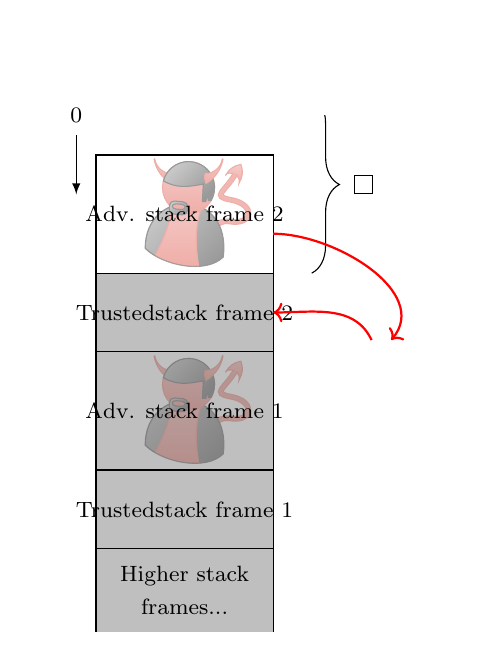
\begin{tikzpicture}[scale=.5, every node={scale=.5}]
      % recurrent parts
      \draw (-0.5,13) node {\footnotesize 0};
      \draw (-0.5,12.5) edge[thin,-latex] (-0.5,11);
      \stdstackstart[13]
      \inactsf{(0,2)}{(4.5,4)} {\footnotesize Trusted\\ \footnotesize stack frame 1}
      \inactadv{(0,4)}{(4.5,7)} {\footnotesize Adv. stack frame 1}
      \inactsf{(0,7)}{(4.5,9)} {\footnotesize Trusted \\ \footnotesize stack frame 2}
      \actadv{(0,9)}{(4.5,12)} {\footnotesize Adv. stack frame 2}

      % Stack pointer 1
      \begin{scope}
        \clip (4.6,4) rectangle (9,13);
        \capbracebot{(4.6,4)}{(4.6,13.5)}{adv. stack\\\footnotesize cap. 1}
      \end{scope}
      Stack pointer 2
      \begin{scope}
        \clip (4.8,4) rectangle (9,13);
        \capbrace{(5.2,9)}{(5.2,13.5)}{adv. stack\\\footnotesize cap. 2}
      \end{scope}

      \draw[red,thick,->] (4.5,10) to[out=0,in=50] node[midway,right] {} (7.5,7.3);
      \draw[red,thick,->] (7,7.3) to[out=115,in=0] node[midway,right] {} (4.5,8);
    \end{tikzpicture}
    \caption{An adversary uses a previous stack frame's stack pointer.}
    \label{fig:stack-ptr-abuse}
  \end{subfigure}
  \begin{subfigure}{0.18\linewidth}
    \phantom{testtestes}
  \end{subfigure}
  \begin{subfigure}{0.4\linewidth}
    \centering
    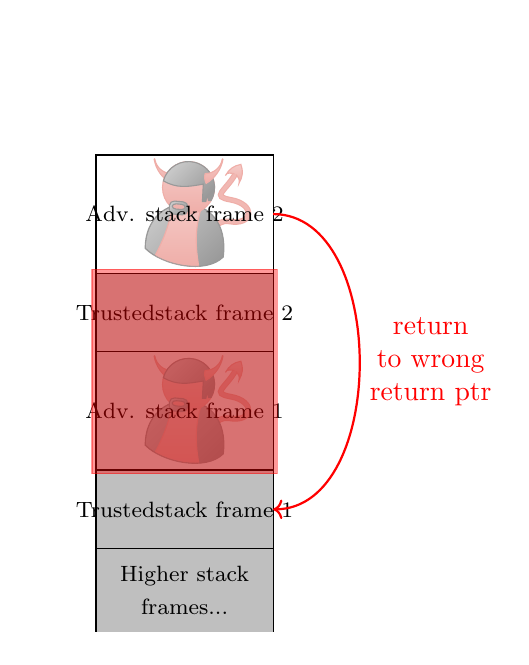
\begin{tikzpicture}[scale=.5, every node={scale=.5}]
      % recurrent parts
      \stdstackstart[13]
      \inactsf{(0,2)}{(4.5,4)} {\footnotesize Trusted\\ \footnotesize stack frame 1}
      \inactadv{(0,4)}{(4.5,7)} {\footnotesize Adv. stack frame 1}
      \inactsf{(0,7)}{(4.5,9)} {\footnotesize Trusted \\ \footnotesize stack frame 2}
      \actadv{(0,9)}{(4.5,12)} {\footnotesize Adv. stack frame 2}
      \fill[red,draw=red,opacity=.4] (-.1,3.9) rectangle (4.6,9.1);
      \draw[red,thick,->] (4.5,10.5) to[out=0,in=0] node[midway,right,align=center] {return\\ to wrong\\ return ptr} (4.5,3);
    \end{tikzpicture}
    \caption{An adversary jumps to a previous stack frame's stack pointer.}
    \label{fig:ret-ptr-abuse}
  \end{subfigure}
  
  \caption{Possible ways to abuse stack and return capabilities}
  \label{fig:stack-ret-ptr-abuse}
\end{figure}

Our StackTokens calling convention is based on a traditional single stack, shared between all components.
As we are on a capability machine, it is natural to add some extra protection to stack and return pointers.
First, we replace stack pointers with stack capabilities.
When a new stack frame is created, the caller provisions it with a stack capability, restricted to the appropriate range, i.e.\ it does not cover the caller's stack frame.
Return pointers, on the other hand, are replaced by a pair of sealed return capabilities.
% KJAA: Again with the sealed pair. Again, this idea is unclear.
They form an opaque closure that the callee can only jump to, and the caller's data becomes available to the caller's return code. 

%informally explain how an adversary may try to abuse stack and return caps
While the above adds extra protection, it is important to understand that it is not sufficient for enforcing WBCF and LSE.
While adversaries only get access to capabilities that they are allowed to use during the stack frame, they have ways to store these capabilities and use them when they are no longer allowed to do so.
Figure~\ref{fig:stack-ret-ptr-abuse} illustrates two examples of this.
In both examples our component and some adversarial component have been taking turns calling each other, so the stack now contains four stack frames alternating between ours and theirs.
The figure on the left (Figure~\ref{fig:stack-ptr-abuse}) illustrates how we try to ensure LSE by restricting the stack capability to the unused part before every call to the adversary.
However, restricting the stack capability does not help when we in the first call give access to the part of the stack where our second stack frame will reside as nothing prevents the adversary from duplicating and storing the stack pointer.
Generally speaking, we have no reason to ever trust a stack capability received from a component we do not trust as that stack capability may have been duplicated and stored for later use.
In the figure on the right (Figure~\ref{fig:ret-ptr-abuse}), we have given the adversary two pairs of sealed return capabilities, one in each of the two calls to the adversarial component.
The adversary may have stored the pair of sealed return capabilities from the first call in order to use it in the second call where they are not allowed to use it.
The figure illustrates how the adversarial code uses the return pair from the first call to return from the second call and thus break WBCF.

\todo[inline]{If target cap. machine is introduced before this section, then revisit/delete this section.}
% Informally explain how we prevent this using linear capabilities
As the examples illustrate, the standard memory and object-like capabilities (sealed capabilities) do not provide sufficient guarantees to enforce LSE and WBCF.
The two properties can be enforced with a calling convention that utilizes the guarantees of linear capabilities.
% What is linear capabilities, split/splice
A linear capability is a capability with no alias that cannot be duplicated.
This is enforced dynamically on the capability machine, so when a linear capability is moved between registers or stored to memory, the source register is cleared, and when a linear capability is read from memory, the source address is cleared.
A capability machine with linear capabilities also needs special instructions to split and splice.
Split and splice do exactly what their names suggest: Split splits a capability into two capabilities with the same permissions and with ranges that are disjointed and sum up to the range of the original capability, and splice does the inverse.

% Stack capability linear
The linear capabilities are put to use by requiring the stack capability to be linear.
On call, the caller splits the stack capability in two, such that they have a capability for their local stack frame and a capability for the unused part of the stack.
The stack capability for their local stack frame is sealed and used as the data part of the sealed return pair, and the stack capability for the remainder of the stack is given to the callee.
% Prevention of left attack non-aliasing of linear capabilities - token like (ensuring LSE)
Because the stack capability is linear the caller knows that the capability for their local stack frame cannot have an alias.
This means that an adversary will need the stack capability the caller produced in order to access their local data.
While the caller gives the capability to the adversary, it is only after the caller seals it which makes the capability opaque.
This is illustrated in Figure~\ref{fig:stack-ptr-abuse-prev} and prevents the issue illustrated in Figure~\ref{fig:stack-ptr-abuse}.

% Prevention of attack 2
In a traditional calling convention with a single stack, the stack serves as a call stack keeping track of the order calls where made in and thus in which order they should be returned to.
A caller pushes a stack frame to the stack on call and a callee pops a stack frame from the stack upon return.
However without any enforcement, there is nothing to prevent a callee from returning from an arbitrary call on the call stack.
This is exactly what the adversary does in Figure~\ref{fig:ret-ptr-abuse} when they skip two stack frames.
In the presence of adversarial code, we need some enforcement mechanism that allows us to make sure that the order of the call stack is kept.
One way to enforce this would be to hand out a token on call that can only be used when the caller's stack frame is on top of the call stack.
The callee would have to provide this token on return to prove that it is allowed to return to the caller, and on return the token would be taken back by the caller to prevent it from being spent multiple times.
As it turns out, the stack capability for the unused part of the stack can be used as such a token in the following way:
On return the callee has to give back the stack capability they were given on invocation.
When the caller receives a stack capability back on return, they need to check that this token is actually spendable, i.e.\ check whether their stack frame is on top of the call stack.
They do this by attempting to restore the stack capability from before the call by splicing the return token with the stack capability for the local stack frame which at this point has been unsealed again.
If the splice is successful, then the caller knows that the two capabilities are adjacent. On the other hand, if the splice fails, then they are alerted to the fact that their stack frame may not be the topmost.
StackTokens uses this approach, and as illustrated in Figure~\ref{fig:ret-ptr-abuse-prev} it prevents the issue in Figure~\ref{fig:ret-ptr-abuse} as the adversary does not return a spendable token when they return.
\begin{figure}
  \centering
  \begin{subfigure}{0.4\linewidth}
    \centering
    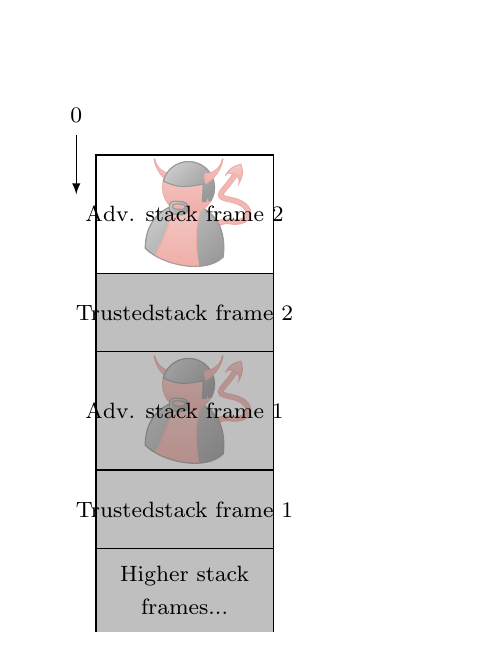
\begin{tikzpicture}[scale=.5, every node={scale=.5}]
      % recurrent parts
      \draw (-0.5,13) node {\footnotesize 0};
      \draw (-0.5,12.5) edge[thin,-latex] (-0.5,11);
      \stdstackstart[13]
      \inactsf{(0,2)}{(4.5,4)} {\footnotesize Trusted\\ \footnotesize stack frame 1}
      \inactadv{(0,4)}{(4.5,7)} {\footnotesize Adv. stack frame 1}
      \inactsf{(0,7)}{(4.5,9)} {\footnotesize Trusted \\ \footnotesize stack frame 2}
      \actadv{(0,9)}{(4.5,12)} {\footnotesize Adv. stack frame 2}

      \lincapbrace{(4.6,2)}{(4.6,4)}{data return\\\footnotesize cap. 1}

      % Stack pointer 1
      \lincapbrace{(4.6,4)}{(4.6,7)}{adv. stack\\\footnotesize cap. 1}
      % return cap
      \lincapbrace{(4.6,7)}{(4.6,9)}{data return\\\footnotesize cap. 2}
     %  Stack pointer 2
      \begin{scope}
        \clip (4.8,4) rectangle (9,13);
        \lincapbrace{(4.6,9)}{(4.6,13.5)}{adv. stack\\\footnotesize cap. 2}
      \end{scope}

    \end{tikzpicture}
    \caption{The non-duplicable linear stack capability for the trusted code's
      stack frame and the opacity of sealed capabilities ensures LSE.}
    \label{fig:stack-ptr-abuse-prev}
  \end{subfigure}
  \begin{subfigure}{0.18\linewidth}
    \phantom{testtestes}
  \end{subfigure}
  \begin{subfigure}{0.4\linewidth}
    \centering
    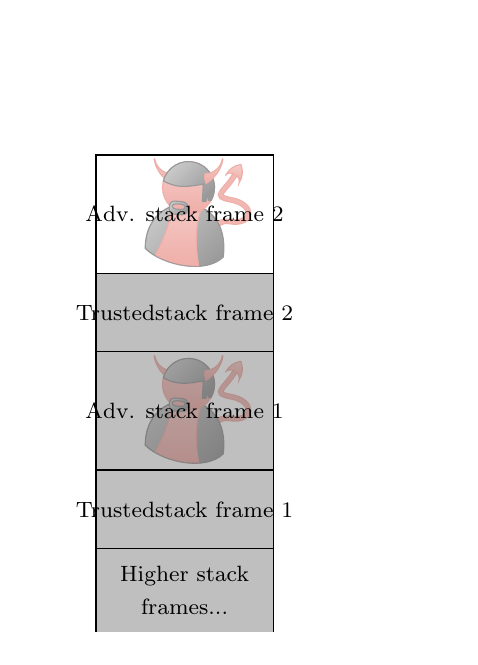
\begin{tikzpicture}[scale=.5, every node={scale=.5}]
      % recurrent parts
      \stdstackstart[13]
      \inactsf{(0,2)}{(4.5,4)} {\footnotesize Trusted\\ \footnotesize stack frame 1}
      \inactadv{(0,4)}{(4.5,7)} {\footnotesize Adv. stack frame 1}
      \inactsf{(0,7)}{(4.5,9)} {\footnotesize Trusted \\ \footnotesize stack frame 2}
      \actadv{(0,9)}{(4.5,12)} {\footnotesize Adv. stack frame 2}

      \lincapbrace{(4.6,2)}{(4.6,4)}{data return\\\footnotesize cap. 1}

     %  Stack pointer 2
      \begin{scope}
        \clip (4.8,4) rectangle (9,13);
        \lincapbrace{(4.6,9)}{(4.6,13.5)}{adv. stack\\\footnotesize cap. 2}
      \end{scope}

      \redcross{(5,4)}
    \end{tikzpicture}
    \caption{The trusted caller fails to splice the stack capability returned by
    the adversary with the capability for the trusted caller's local stack frame.}
    \label{fig:ret-ptr-abuse-prev}
  \end{subfigure}
  \caption{}
\end{figure}

% Non-empty trusted stack frames.
In order for a call to have a presence on the call stack, its stack frame must be non-empty.
If we could have empty stack frames on the call stack, then it would be impossible to tell whether the topmost non-empty stack frame has an empty stack frame on top of it.
Non-empty stack frames come naturally in traditional C-like calling convention as they keep track of old stack pointers and old program counters on the stack, but in StackTokens these things are part of the return pair which means that a caller with no local data may only need an empty stack frame.
This means that a caller using StackTokens needs to take care that their stack frame is non-empty in order to reserve their spot in the return order.
There is also a more practical reason for a StackTokens caller to make sure their stack frame is non-empty: They need a bit of the stack capability in order to perform the splice that verifies the validity of the return token.

% known stack base
% + more
At this point, the caller checks that the return token is adjacent to the stack capability for the caller's local stack frame and they have the means to do so.
However, this does not make sure that the caller's stack frame is on top of the call stack.
The issue is that stack frames may not be tightly packed leaving space between stack frames in memory.
An adversarial callee may even intentionally leave a bit of space in memory above the caller's stack frame, so that they later can return out of order by returning the bit of the return token for the bit of memory left above the caller's stack frame.
This is illustrated in Figure~\ref{fig:stk-base-abuse}: In Figure~\ref{fig:stack-base-abuse-a}, a trusted caller has called an adversarial callee.
The adversary calls the trusted code back, but first they split the return token in two and store on the heap the part for the memory adjacent to the trusted caller's call frame (Figure~\ref{fig:stack-base-abuse-b}).
The trusted caller calls the adversary back using the precautions we have described so far (Figure~\ref{fig:stack-base-abuse-c}).
At this point (Figure~\ref{fig:stack-base-abuse-b})), the adversary has access to a partial return token adjacent to the trusted caller's first stack frame which allows the adversary to return from this call breaking WBCF.
For the caller to be sure that there are no hidden stack frames above its own, they need to make sure that the return token is exactly the same as the one they passed to the callee.
In StackTokens, the caller verifies the validity of the return token by checking whether the base address\footnote{The stack grows downwards in the address space} of a returned token corresponds to the base address of the return token they gave to the callee.
In the scenario we just sketched, the caller would be alerted to the attempt to break WBCF when the base address check of the return token fails in Figure~\ref{fig:stack-base-abuse-d}.

% Where do we get the stack pointer from, how can we know it is linear
% The other attack.
% KJAA: It is unclear to me what 'at this point' refers to.
At this point, the caller is able to verify whether a return token is spendable which allows them to decide whether they have the topmost stack frame on a call stack.
However, in order to have WBCF there should only be one call stack, so the caller should also be able to verify that they have the top stack frame on the call stack used by all well-behaved components.
In case a trusted component did not start the execution on the machine, i.e.\ they were called by another component, then the trusted component has no way to be sure whether the stack capability passed to them corresponds to the one and only call stack.
To illustrate how an adversarial component can break WBCF by using multiple different stack capabilities consider this example: An adversary calls a trusted component with a callback and some linear capability that they claim is the stack capability.
The trusted component executes using the stack capability given to them and at some point they invoke the callback, creating return tokens and so on.
The adversary stores the return pair and return token and calls another trusted component but with a new callback and a new linear capability that they claim is the stack capability.
Again, this trusted component also executes using the stack capability given to them and at some point they too invoke the callback, taking all the precautions we have described so far.
At this point, the adversary has everything they need to return from either of the two callbacks.
Specifically, they could return from the first callback invocation before they have returned from the second, breaking WBCF.
From a high-level perspective, the problem is that both trusted components will be able to verify that they have the top stack frame on the call stack.
They are both correct as the adversarial component has created two call stacks, one for each of the components.
In order to solve this problem, the well-behaved code needs to somehow agree on the call stack.
We do this by statically deciding on a global base address for the stack which is used for the entirety of the execution.
A caller makes sure that they are using the correct stack by checking that the base address of the stack capability they receive corresponds to the global stack base address.
This also means that on every return, the caller will check whether the return token's base address is equal to the global stack address.

Having a globally decided stack address also solves another challenge.
Namely, the stack capability has to be linear in order for a caller to use it as a token, so a caller has to make sure that a capability is in fact linear when it is proposed as the stack capability by an untrusted source.
This is, however, implicitly checked when the caller checks that the stack capability governs the global stack base address.
The reason is that the stack capability needs to start execution as a linear capability which means that the capability that governs the global stack base address to begin with is linear.
Due to the non-duplicability of linear capability and the fact that they cannot become non-linear during execution, the caller knows that if they have a capability that governs the global stack base address, then it must be linear.

% Return pointers/return seals
The return pointer in the StackToken scheme is a pair of sealed capabilities where the code part of the pair is the old program counter, and the data part is the stack capability for the local stack frame of the caller.
Both of the capabilities in the pair are of course sealed with the same seal.
% One seal per return point
All call points need to be associated with a unique seal (a return seal) that is only used to seal the capabilities in the return pair for that particular call point.
The return seal is what associates the stack frame on the call stack with a specific call point in a program, so if we allowed return seals to be reused, it would be possible to return to a different call point than the one that caused the stack frame to be pushed on the call stack which would break WBCF.
For similar reasons, we cannot allow return seals to be used to seal closures.
% Don't be stupid
Return seals should never be leaked to adversarial code as this would allow them to unseal the local stack frame of a caller breaking LSE.
This goes for direct leaks, such as leaving a seal in a register or writing it to adversarial memory, as well as indirect leaks, where a capability for reading a return seal (either directly or indirectly) from memory is leaked.

% Note about them vs us, we do nothing that they couldn't do
In the description of the StackToken calling scheme, it has sometimes been in terms of ``them vs us''.
This may have created the impression of an asymmetric calling convention that places a special status on trusted components allowing them to protect themselves against adversaries.
However, StackTokens is a modular calling scheme no restriction is put on adversarial components that we do not expect trusted components to meet.
This means that any component can ensure WBCF and LSE by employing StackTokens.
% KJAA: ^-- Assuming that there is a global stack address capability, no? Can I "suddenly" begin to impose StackTokens?

% Summary of CC
In the this section, we have described our proposed calling convention, StackTokens.
In this paragraph we summarize it:
\begin{description}
\item[Check the base address of the stack capability before and after calls] 
\item[Make sure that local stack frames are non-empty]
\item[Create token and data return capability on call] split the stack capability in two to get a stack capability for you local stack frame and a stack capability for the unused part of the stack. The stack capability for your local stack frame is sealed and used for the data part of the return pair.
\item[Create code return capability on call] Seal the old program pointer.
\item[Reasonable use of seals] return seals are only used to seal old program pointers, all return seals are only used for one call site, and return seals are not leaked.
\end{description}

\begin{figure}
  \centering
  \begin{subfigure}{0.23\linewidth}
    \centering
    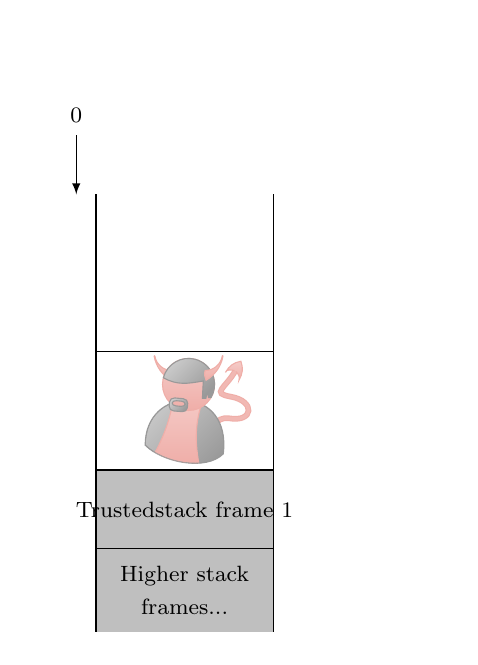
\begin{tikzpicture}[scale=.5, every node={scale=.5}]
      % recurrent parts
      \draw (-0.5,13) node {\footnotesize 0};
      \draw (-0.5,12.5) edge[thin,-latex] (-0.5,11);
      \stdstackstart[13]
      \inactsf{(0,2)}{(4.5,4)} {\footnotesize Trusted\\ \footnotesize stack frame 1}
      \actadv{(0,4)}{(4.5,7)}{}

      \lincapbrace{(4.6,2)}{(4.6,4)}{}
      \begin{scope}
        \clip (4.8,1) rectangle (9,13);
      \lincapbracebot{(4.6,4)}{(4.6,13.5)}{}
      \end{scope}

    \end{tikzpicture}
    \caption{}
    \label{fig:stack-base-abuse-a}
  \end{subfigure}
  \begin{subfigure}{0.24\linewidth}
    \centering
    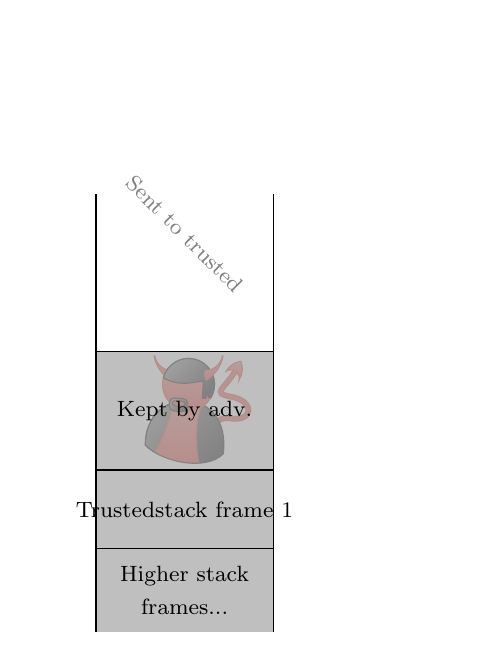
\begin{tikzpicture}[scale=.5, every node={scale=.5}]
      % recurrent parts
      \stdstackstart[13]
      \inactsf{(0,2)}{(4.5,4)} {\footnotesize Trusted\\ \footnotesize stack frame 1}
      \inactadv{(0,4)}{(4.5,7)}{\footnotesize Kept by adv.}
      \node[opacity=0.5,rotate=-45] at (2.25,10) {\footnotesize Sent to trusted};
      \lincapbrace{(4.6,2)}{(4.6,4)}{}
      \lincapbrace{(4.6,4)}{(4.6,7)}{}
      
      \begin{scope}
        \clip (4.8,1) rectangle (9,13);
      \lincapbracebot{(4.6,7)}{(4.6,13.5)}{}
      \end{scope}

    \end{tikzpicture}
    \caption{}
    \label{fig:stack-base-abuse-b}
  \end{subfigure}
  \begin{subfigure}{0.24\linewidth}
    \centering
    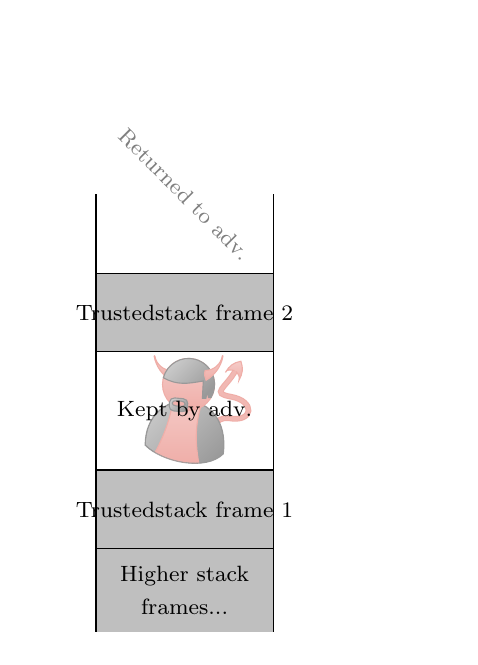
\begin{tikzpicture}[scale=.5, every node={scale=.5}]
      % recurrent parts
      \stdstackstart[13]
      \inactsf{(0,2)}{(4.5,4)} {\footnotesize Trusted\\ \footnotesize stack frame 1}
      \actadv{(0,4)}{(4.5,7)}{\footnotesize Kept by adv.}
      \inactsf{(0,7)}{(4.5,9)} {\footnotesize Trusted\\ \footnotesize stack frame 2}
      \node[opacity=0.5,rotate=-45] at (2.25,11) {\footnotesize Returned to adv.};
      \lincapbrace{(4.6,2)}{(4.6,4)}{}
      \lincapbrace{(4.6,4)}{(4.6,7)}{}
      \lincapbrace{(4.6,7)}{(4.6,9)}{}
      \begin{scope}
        \clip (4.8,1) rectangle (9,13);
        \lincapbracebot{(4.6,9)}{(4.6,13.5)}{}
      \end{scope}

    \end{tikzpicture}
    \caption{}
    \label{fig:stack-base-abuse-c}
  \end{subfigure}
  \begin{subfigure}{0.24\linewidth}
    \centering
    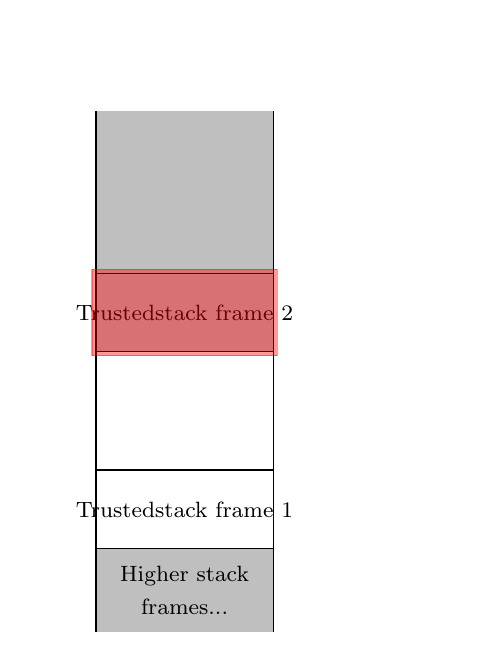
\begin{tikzpicture}[scale=.5, every node={scale=.5}]
      % recurrent parts
      \stdstackstart[13]
      \actsf{(0,2)}{(4.5,4)} {\footnotesize Trusted\\ \footnotesize stack frame 1}

      \inactsf{(0,7)}{(4.5,9)} {\footnotesize Trusted\\ \footnotesize stack frame 2}
      \begin{scope}
        \clip (-.1,-.1) rectangle (4.6,13.1);
        \draw[fill=gray!50] (0,9) rectangle (4.5,13.5);
      \end{scope}

      \lincapbrace{(4.6,2)}{(4.6,7)}{}
      \lincapbrace{(4.6,7)}{(4.6,9)}{}

      \fill[red,draw=red,opacity=.4] (-.1,6.9) rectangle (4.6,9.1);
      \begin{scope}
        \clip (4.8,1) rectangle (9,13);
        \lincapbracebot{(4.6,9)}{(4.6,13.5)}{}
      \end{scope}

    \end{tikzpicture}
    \caption{}
    \label{fig:stack-base-abuse-d}
  \end{subfigure}
  \caption{}
  \label{fig:stk-base-abuse}
\end{figure}


% \begin{itemize}
% \item informally explain how an adversary may try to abuse stack and return caps
% \item informally explain how we prevent this using linear capabilities
% \item use the tikz pictures from the PriSC presentation to explain all of this
% \end{itemize}

\section{Formulating Security with a Fully Abstract Overlay Semantics}
\label{sec:form-secur-with}
\begin{figure}[htb]
  \centering
  \[
    \arraycolsep=1.4pt
    \begin{array}{rcl}
      \src{\SealableCaps} & \defbnf& \SealableCaps \mid \src{\stkptr{\permbnf,\basebnf,\aendbnf,\addrbnf}} \mid \src{\retptrd(\basebnf,\aendbnf)}\\
                          & &  \mid \src{\retptrc(\basebnf,\aendbnf,\addrbnf)}\\
      \multicolumn{3}{c}{
      \begin{array}{lcrclcr}
        \src{\StkFrame} & \defeq & \src{\Addr \times \MemSeg} & \phantom{skipskipsip} & \src{\Stack} & \defeq & \src{ \StkFrame^*}
      \end{array}
                                                                                                                }\\
      \src{\ExecConf} & \defeq & \Mem \times \Reg \; \src{\times \; \Stack \times \MemSeg} \\
    \end{array}
  \] 
\[
  \begin{array}{rcl}
    \offpc,\offsigma & \in & \nats \\
    \src{\Instr} & \defbnf &  \Instr \mid \scall{\offpc,\offsigma}{r}{r}
  \end{array}
\]
  \caption{The syntax of the capability machine with a built-in stack.}
  \label{fig:src-syntax}
\end{figure}

\begin{figure}[htb]
  \centering
  \label{fig:src-op-sem}
  \caption{An excerpt of the operational semantics of the capability machine with a built-in stack.}
\end{figure}


\begin{itemize}
\item present our source language, its operational semantics (excerpts)
\item mention our assumption of reasonability
\item present the full abstraction theorem.
\end{itemize}

\section{Proving full abstraction}
\label{sec:fa-proof}

\begin{itemize}
\item Logical relation
\item FTLR
\item Sketch high-level structure of the proof
\end{itemize}

\section{Discussion}
\label{sec:discussion}
\begin{itemize}
\item mention that tail calls are supported through xjmp
\item explain how fully abstract overlay semantics could form one pass of a verified secure compiler.
\item Performance?  Implementability of linear caps?
\item Sharing stack references accross component boundaries is supported
\item Other notions of well-bracketedness (specifically one would be to allow different stacks)
\end{itemize}

\section{Related Work}

In this section, we discuss related work on securely enforcing control flow correctness and/or local state encapsulation.
We do not repeat the work we discussed in Section~\ref{sec:introduction}.

Capability machines originate with \citet{dennis_programming_1966} and we refer to \citet{levy_capability-based_1984} and \citet{watson_cheri:_2015} for an overview of previous work.
The capability machine formalized in Section~\ref{sec:cap-mach-w-seal-and-lin} is modeled after CHERI~\citep{watson_cheri:_2015,woodruff_cheri_2014}.
This is a recent and relatively mature capability machine, which combines capabilities with a virtual memory approach, in the interest of backwards compatibility and gradual adoption.
For simplicity, we have omitted features of CHERI that were not needed for modelling StackTokens (e.g.\ local capabilities, virtual memory).

Plenty of other papers enforce well-bracketed control flow at a low level, but most are restricted to preventing particular types of attacks and enforce only partial correctness of control flow.
This includes particularly the line of work on \emph{control-flow integrity}~\citep{abadi_control-flow_2005}.
This technique prevents certain classes of attacks by sanitizing addresses before direct and indirect jumps based on static information about a program's control graph and a shadow stack.
Contrary to StackTokens, CFI can be implemented on commodity hardware rather than capability machines.
However, its attacker model is different and its security goals are weaker.
They assume an attacker that is not able to execute code, but can overwrite arbitrary data at any time during execution (to model buffer overflows).
In terms of security goals, the technique does not enforce local stack encapsulation.
Also, it only enforces a weak form of control flow correctness, saying that jumps stay within the static control flow graph of a program~\cite{Abadi2005Theory}.
Such a property ignores temporal properties and seems hard to use for reasoning.
There is also more and more evidence that these partial security properties are not enough to prevent realistic attacks in practice~\citep{Evans:2015:CJW:2810103.2813646,Carlini2015ControlFlowBending}.

More closely related to our work are papers that use separate per-component stacks, a trusted stack manager and some form of memory isolation to enforce control-flow correctness as part of a secure compilation result~\citep{patrignani_modular_2016,juglaret_beyond_2016}.
Our work differs from theirs in that we use a different low-level security primitive (a capability machine with local capabilities rather than a machine with a primitive notion of compartments) and we do not use per-component stacks or a trusted stack manager, but a single shared stack and a decentralized calling convention based on linear capabilities.
Both prove a secure compilation result from a high-level language, which clearly implies a general form of control-flow correctness, but that result is not separated from the results about other aspects of their compiler.

CheriBSD applies a similar approach with separate per-component stacks and a trusted stack manager on a capability machine~\cite{watson_cheri:_2015}.
The authors use local capabilities to prevent components from accidentally leaking their stack pointer to other components, but there is no actual capability revocation at play.
They do not provide many details on this mechanism and it is, for example, not clear if and how they intend to deal with higher-order interfaces (C function pointers) or stack references shared accross component boundaries. 

The fact that our full abstraction result only applies to reasonable components (see Section~\ref{sec:form-secur-with}) makes it related to full abstraction results for unsafe languages.
In their study of compartmentalization primitives, \Citet{juglaret_beyond_2016} discuss the property of Secure Compartmentalizing Compilation (SCC): a variant of full abstraction that applies to unsafe source languages.
Essentially, they modify standard full abstraction so that preservation and reflection of contextual equivalence are only guaranteed for components that are {\itshape fully defined}, which means essentially that they do not exhibit undefined behavior in any fully defined context.
In follow-up work, \citet{DBLP:journals/corr/abs-1802-00588} extend this approach to scenarios where components only start to exhibit undefined behavior after a number of well-defined steps.
If we see reasonable behavior as defined behavior, then our full abstraction result can be seen as an application of this same idea.
Our results do not apply to dynamic compromise scenarios because they are intended to be used in the verification of a secure compiler, where these scenarios are not relevant.

\bibliography{references}


%% Appendix
% \appendix
% \section{Appendix}

% Text of appendix \ldots

\end{document}
 